\documentclass[nooutcomes]{ximera}
%\documentclass[space,handout,nooutcomes]{ximera}

% For preamble materials

\usepackage{pgf,tikz}
\usepackage{mathrsfs}
\usetikzlibrary{arrows}
\usepackage{framed}
\usepackage{amsmath}
\pgfplotsset{compat=1.17}

\def\fixnote#1{\begin{framed}{\textcolor{red}{Fix note: #1}}\end{framed}}  % Allows insertion of red notes about needed edits
%\def\fixnote#1{}

\def\detail#1{{\textcolor{blue}{Detail: #1}}}   

\pdfOnly{\renewenvironment{image}[1][]{\begin{center}}{\end{center}}}

\graphicspath{
  {./}
  {chapter1/}
  {chapter2/}
  {chapter4/}
  {proofs/}
  {graphics/}
  {../graphics/}
}

\newenvironment{sectionOutcomes}{}{}


%%% This set of code is all of our user defined commands
\newcommand{\bysame}{\mbox{\rule{3em}{.4pt}}\,}
\newcommand{\N}{\mathbb N}
\newcommand{\C}{\mathbb C}
\newcommand{\W}{\mathbb W}
\newcommand{\Z}{\mathbb Z}
\newcommand{\Q}{\mathbb Q}
\newcommand{\R}{\mathbb R}
\newcommand{\A}{\mathbb A}
\newcommand{\D}{\mathcal D}
\newcommand{\F}{\mathcal F}
\newcommand{\ph}{\varphi}
\newcommand{\ep}{\varepsilon}
\newcommand{\aph}{\alpha}
\newcommand{\QM}{\begin{center}{\huge\textbf{?}}\end{center}}

\renewcommand{\le}{\leqslant}
\renewcommand{\ge}{\geqslant}
\renewcommand{\a}{\wedge}
\renewcommand{\v}{\vee}
\renewcommand{\l}{\ell}
\newcommand{\mat}{\mathsf}
\renewcommand{\vec}{\mathbf}
\renewcommand{\subset}{\subseteq}
\renewcommand{\supset}{\supseteq}
%\renewcommand{\emptyset}{\varnothing}
%\newcommand{\xto}{\xrightarrow}
%\renewcommand{\qedsymbol}{$\blacksquare$}
%\newcommand{\bibname}{References and Further Reading}
%\renewcommand{\bar}{\protect\overline}
%\renewcommand{\hat}{\protect\widehat}
%\renewcommand{\tilde}{\widetilde}
%\newcommand{\tri}{\triangle}
%\newcommand{\minipad}{\vspace{1ex}}
%\newcommand{\leftexp}[2]{{\vphantom{#2}}^{#1}{#2}}

%% More user defined commands
\renewcommand{\epsilon}{\varepsilon}
\renewcommand{\theta}{\vartheta} %% only for kmath
\renewcommand{\l}{\ell}
\renewcommand{\d}{\, d}
\newcommand{\ddx}{\frac{d}{dx}}
\newcommand{\dydx}{\frac{dy}{dx}}


\usepackage{bigstrut}


%\usepackage{tikz}


\title{Symmetry}
\author{Bart Snapp and Brad Findell}
\begin{document}
\begin{abstract}
Short-answer questions about symmetry. 
\end{abstract}
\maketitle

\begin{question}
Categorize the capital letters of the alphabet by their symmetries.  Use the following font: 
\begin{image}
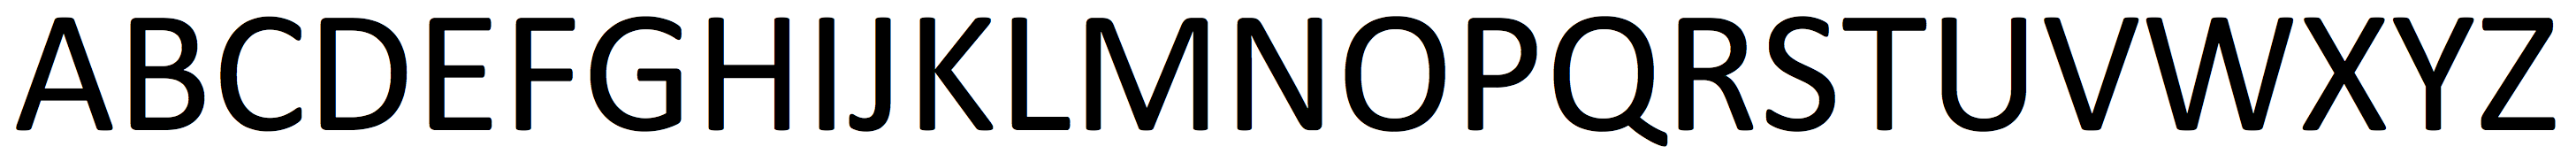
\includegraphics[scale=0.35]{alphabet.png}
\end{image}
%\begin{tikzpicture}
%  \node {\scalebox{10}{\textsf{K}}};
%\end{tikzpicture}
\begin{question}
Vertical line symmetry:  $\answer{AHIMOTUVWXY}$
\begin{feedback}[attempt]
Enter \textbf{capital} letters in any order, without space.
\end{feedback}
\end{question}
\begin{question}
Horizontal line symmetry:  $\answer{CDEHIOX}$  
\begin{feedback}[attempt]
Be careful about B and K.  
\end{feedback}
\begin{feedback}[correct]
In some fonts, B and K have horizontal line symmetry.  In this one, the B is slightly bigger on the bottom.  
\end{feedback}
\end{question}
\begin{question}
$180^\circ$ rotational symmetry: $\answer{HINOSXZ}$
\begin{feedback}[correct]
In this font, the O is slightly taller than it is wide.  If it were a circle, it would have much more symmetry.
\end{feedback}
\end{question}
\begin{question}
None: $\answer{BFGJKLPQR}$
\end{question}
\end{question}

\begin{question}
Write the words COKE and PEPSI in capital letters so that they read vertically.  Use a mirror to look at a reflection of the words.  Which word can appear the same on a soda can as in a mirror?  $\answer[format=string]{COKE}$
\begin{question}
\textbf{Explanation:} If the K is symmetric in the font, then all the letters in COKE have $\answer[format=string]{horizontal line symmetry}$ (three words), which becomes vertical line symmetry when the word is written vertically. PEPSI, on the other hand, has several letters without that symmetry.  
\end{question}
\end{question}


\begin{question}
We often say a figure is ``symmetric'' when we notice that it has symmetry, but now we want to be more precise:  

A \emph{symmetry} of a figure is a
\wordChoice{\choice{reflection}\choice{rotation}\choice[correct]{transformation}\choice{translation}} 
that maps a figure 
\wordChoice{\choice{to its opposite}\choice[correct]{onto itself}\choice{to another figure}}.  
\end{question}

\begin{question}
Is a sequence of two symmetries of a figure also a symmetry of that figure?
$\answer[format=string]{Yes}$.
\begin{question}
%If a transformation T1 maps a figure onto itself and another transformation T2 maps the figure onto itself, then T1 followed by T2 also maps the figure onto itself.  
\textbf{Explanation:} The first transformation maps the figure onto itself, and the second transformation maps the figure onto itself, so the sequence of two transformations maps the figure $\answer[format=string]{onto itself}$.  
\end{question}
\end{question}

\begin{question}
Is the identity transformation a symmetry of \emph{any} figure? 
$\answer[format=string]{Yes}$.
\begin{feedback}[correct]
If the identity transformation is the \emph{only} symmetry of a figure, we usually say the figure is asymmetric or has no symmetry.  
\end{feedback}
\begin{question}
\textbf{Some possible explanations:} 
\begin{itemize}
\item The identity transformation satisfies the definition of a symmetry: It maps the figure $\answer[format=string]{onto itself}$ (two words). 
\item If a figure has reflection symmetry $R_k$ about a line $k$, then $R_k$ followed by $R_k$ is the $\answer[format=string]{identity transformation}$ (two words).  And by the previous result, this sequence of symmetries must also be a symmetry.  
\item If a figure has rotational symmetry $R_\alpha$ by some angle $\alpha$ about some center, then it must also have a rotational symmetry $R_{-\alpha}$ by the angle $-\alpha$ about the same center.  $R_\alpha$ followed by $R_{-\alpha}$ is the $\answer[format=string]{identity transformation}$ (two words).  And by the previous result, this sequence of symmetries must also be a symmetry.  
\end{itemize}
\end{question}
\end{question}

\begin{question}
It is reasonable to call the identity transformation a translation because it is a translation of magnitude $\answer{0}$ in any direction.  

It is reasonable to call the identity transformation a rotation because it is a rotation of $\answer{0}$ degrees about any center.  
\end{question}

\begin{question}
Indicate the number of rotation and reflection symmetries of the following figures (including the identity rotation): 
\begin{enumerate}
\item An equilateral triangle: $\answer{3}$ rotation(s) and $\answer{3}$ reflection(s). 
\item An isosceles triangle that is not equilateral: $\answer{1}$ rotation(s) and $\answer{1}$ reflection(s).
\item A square: $\answer{4}$ rotation(s) and $\answer{4}$ reflection(s).
\item A rectangle that is not a square: $\answer{2}$ rotation(s) and $\answer{2}$ reflection(s).
\item A rhombus that is not a square: $\answer{2}$ rotation(s) and $\answer{2}$ reflection(s).
\item A (non-special) parallelogram: $\answer{2}$ rotation(s) and $\answer{0}$ reflection(s).
\item A regular $n-$gon: $\answer{n}$ rotation(s) and $\answer{n}$ reflection(s).
\end{enumerate}
\end{question}

%\begin{question}
%Describe all of the symmetries of the following figures: 
%\begin{enumerate}
%\item An equilateral triangle
%\item An isosceles triangle that is not equilateral
%\item A square
%\item A rectangle that is not a square
%\item A rhombus that is not a square
%\item A (non-special) parallelogram
%\item A regular $n$-gon
%\end{enumerate}
%\end{question}


\begin{question}
Suppose that quadrilateral $ABCD$ has exactly one rotation symmetry (other than the identity transformation) and no reflection symmetry.  What kind(s) of quadrilateral could it be?  

\textbf{Answer:}  It must be a $\answer[format=string]{parallelogram}$.
\begin{question}
\textbf{Explanation:} If a rotation of $\alpha$ is a symmetry of a figure, then a rotation of $2\alpha$ must also be a symmetry.  Thus, for the quadrilateral to have only one (non-identity) rotation symmetry, it must be that $2\alpha$ (but not $\alpha$) is a multiple of 360 degrees.  Therefore $\alpha = \answer{180}$ degrees.  

This rotation will swap opposite vertices, which implies that the center of rotation is the midpoint of each diagonal, so that the diagonals must $\answer[format=string]{bisect}$ each other.  Thus, quadrilateral $ABCD$ is a $\answer[format=string]{parallelogram}$ that is not any more special (or it would have additional symmetry).  
\end{question}
\end{question}

\begin{question}
Suppose that quadrilateral $ABCD$ has exactly one reflection symmetry and no rotation symmetry (other than the identity transformation).  What kind(s) of quadrilateral could it be? (Select all.)
\begin{selectAll} 
\choice{parallelogram}
\choice{rhombus}
\choice{rectangle}
\choice{square}
\choice[correct]{kite}
\choice[correct]{trapezoid}
\end{selectAll}
\begin{question}
\textbf{Explanation:}  A parallelogram has $180^\circ$ rotational symmetry, so quadrilateral $ABCD$ cannot be a parallelogram, which also excludes the special cases: square, rectangle, 
and $\answer[format=string]{rhombus}$.  If the line of symmetry goes through two vertices, it must be a(n) $\answer[format=string]{kite}$ that is not a rhombus.  If the line of symmetry goes through two sides, it must be a(n) $\answer[format=string]{isosceles trapezoid}$ (two words).  
\end{question}
\end{question}

\begin{question}
What are the symmetries of a circle? (Select all.)
\begin{selectAll}
\choice{translation symmetry}
\choice[correct]{rotation symmetry}
\choice[correct]{reflection symmetry}
\end{selectAll}
\begin{question}
\begin{enumerate}
\item A circle has rotation symmetry by any $\answer[format=string]{angle}$ 
about its $\answer[format=string]{center}$.  
\item A circle has reflection symmetry 
about any $\answer[format=string]{line}$ through its $\answer[format=string]{center}$.  
\item A circle does 
not have translation symmetry.  
\end{enumerate}
\end{question}
\end{question}

\begin{question}
How can you use the symmetries of a circle to determine whether a figure is indeed a circle?  
\begin{freeResponse}
\end{freeResponse}
\begin{hint}
Perform any of the symmetry transformations to be sure that the circle is actually mapped onto itself.  
\end{hint}
\end{question}

\begin{question}
What are the symmetries of a line?  
\begin{selectAll}
\choice[correct]{translation symmetry}
\choice[correct]{rotation symmetry}
\choice[correct]{reflection symmetry}
\end{selectAll}
\begin{question}
\begin{enumerate}
\item A line has translation symmetry by a vector of any length \wordChoice{\choice[correct]{parallel}\choice{perpendicular}\choice{opposite}} to the line.   
\item A line has $\answer{180}$ degree rotational symmetry about any point on the line.  
\item A line has reflection symmetry about any line \wordChoice{\choice{parallel}\choice[correct]{perpendicular}\choice{opposite}} to the line.  A line also has reflection symmetry about itself.  
\end{enumerate}
\end{question}
\end{question}

%\begin{question}
%Given a line, describe a rotation symmetry and a reflection symmetry that have the same effect on the line.  How do the corresponding transformations differ in what they do to the surrounding space?  
%\begin{freeResponse}
%\end{freeResponse}
%\begin{hint}
%Given a point $P$ on the line $k$, let $j$ be the unique line through $P$ perpendicular to $k$.  A $180^\circ$ rotation about $P$ and a reflection about $j$ have the same effect on the line $k$, even though those transformations have different effects on the rest of the plane.  
%\end{hint}
%\end{question}

\begin{question}
How can you use the symmetries of a line to determine whether a figure is indeed a line? 
\begin{freeResponse}
\end{freeResponse}
\begin{hint}
Perform any of the symmetry transformations to be sure that the line is actually mapped onto itself.  
\end{hint}
\end{question}

%\begin{question}
%Find some tessellations.  For each tessellation, describe all of its symmetries.  
%\begin{freeResponse}
%\end{freeResponse}
%\begin{hint}
%\end{hint}
%\end{question}



\end{document}
